\documentclass[a4paper,12pt]{article}

\usepackage{amsmath,amssymb,multicol,tikz,enumitem}
\usepackage[margin=2cm]{geometry}
\usetikzlibrary{calc,shapes}

\pagestyle{empty}

\newcommand\N{\mathbf{N}}
\newcommand\Q{\mathbf{Q}}
\newcommand\R{\mathbf{R}}
\newcommand\Z{\mathbf{Z}}

\usepackage{array}
\newcolumntype{P}[1]{>{\centering\arraybackslash}p{#1}}
\newcommand\indd{${}$\hspace{20pt}}

\begin{document}

\begin{center}
\parbox{3.5cm}{\textbf{Data Structures}} \hfill {\bf\Huge Worksheet 4} \hfill \parbox{3.5cm}{\flushright\textbf{BITL2}} \\[5pt]
\rm\small 23 September 2021
\end{center}

\hrule\vspace{2pt}\hrule

\begin{enumerate}

\item \textbf{Warm up:} Answer the following True / False questions.
\begin{enumerate}
\item A doubly linked list of 10 integers take up twice the space of a singly linked list of 10 integers.
\item A circularly linked list can do the same things as a doubly linked list.
\item Positive integers support iterators.
\end{enumerate}

\item This question is about \textbf{queues}, implemented using an array in a wrap-around method. The queue has size 10, and the \texttt{enqueue} and \texttt{dequeue} functions are executed randomly.
\begin{enumerate}
\item If theses functions are excuted 6 times, what are the possible lengths of the queue afterward? What is the average length?
\item Supose the array holding the queue has size 14, and \texttt{enqueue} has a probability of $\frac{3}4$ being executed, and \texttt{dequeue} has a probability of $\frac14$ being executed.
\begin{enumerate}
\item What is the probability the queue will be full after 6 executions? The queue is full if one spot in the array is empty.
\item \textbf{Bonus:} What is the expected value for number of executions at which the queue is full?
\end{enumerate}
\end{enumerate}
\end{enumerate}

\noindent
The next two problems refer to the following uncompiled \texttt{C++} files.
\[
\hspace{-1.5cm}
\scalebox{.6}{
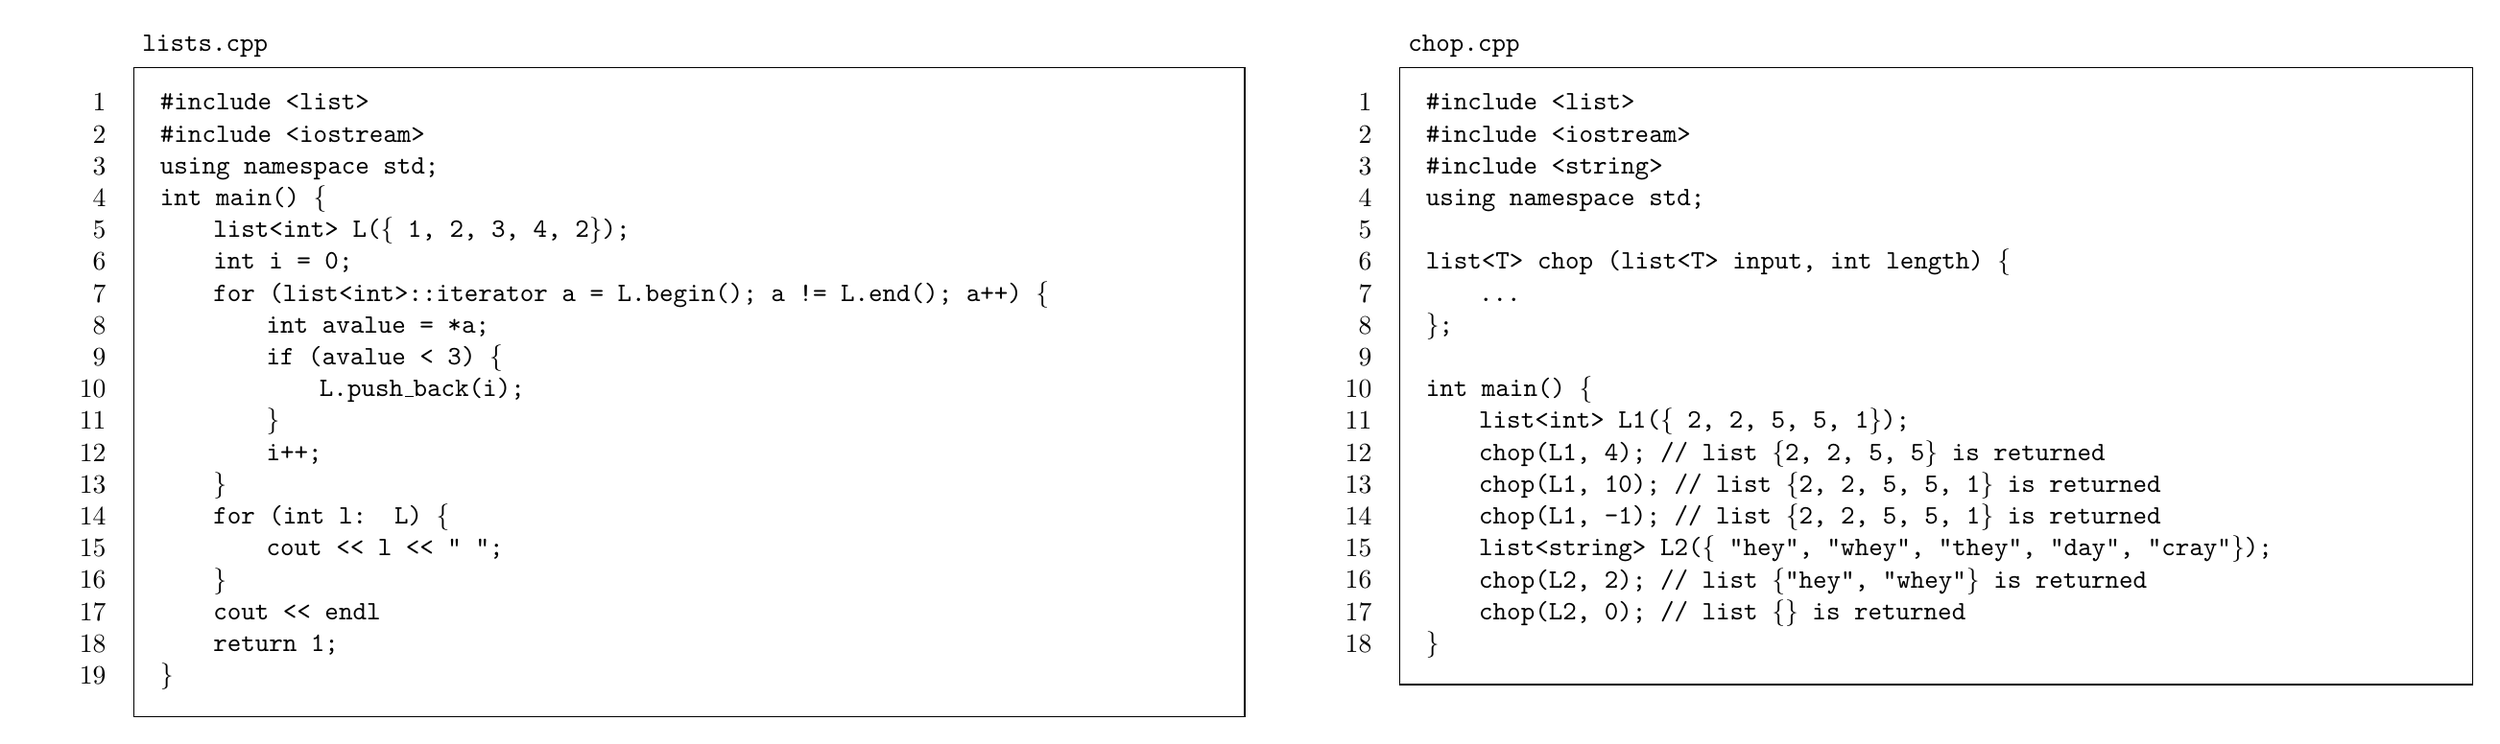
\begin{tikzpicture}
\node[draw,anchor=north,inner sep=10pt] (lists) at (-10,0) {\parbox{14cm}{\raggedright
\texttt{\#include <list>}\linebreak
\texttt{\#include <iostream>}\linebreak
\texttt{using namespace std;}\linebreak
\texttt{int main() \{}\linebreak
\indd\texttt{list<int> L(\{ 1, 2, 3, 4, 2\});}\linebreak
\indd\texttt{int i = 0;}\linebreak
\indd\texttt{for (list<int>::iterator a = L.begin(); a != L.end(); a++) \{}\linebreak
\indd\indd\texttt{int avalue = *a;}\linebreak
\indd\indd\texttt{if (avalue < 3) \{}\linebreak
\indd\indd\indd\texttt{L.push\_back(i);}\linebreak
\indd\indd\texttt{\}}\linebreak
\indd\indd\texttt{i++;}\linebreak
\indd\texttt{\}}\linebreak
\indd\texttt{for (int l: L) \{}\linebreak
\indd\indd\texttt{cout << l << " ";}\linebreak
\indd\texttt{\}}\linebreak
\indd\texttt{cout << endl}\linebreak
\indd\texttt{return 1;}\linebreak
\texttt{\}}
}};
\node[anchor=south west] at (lists.north west) {\texttt{lists.cpp}};
\node[anchor=north,inner sep=10pt,anchor=north east] at (lists.north west) {\parbox{.7cm}{\raggedleft
1\linebreak 2\linebreak 3\linebreak 4\linebreak 5\linebreak 6\linebreak 7\linebreak 8\linebreak 9\linebreak10\linebreak11\linebreak12\linebreak13\linebreak14\linebreak15\linebreak16\linebreak17\linebreak18\linebreak19}};

\node[draw,anchor=north,inner sep=10pt] (chop) at (6.5,0) {\parbox{13.5cm}{\raggedright
\texttt{\#include <list>}\linebreak
\texttt{\#include <iostream>}\linebreak
\texttt{\#include <string>}\linebreak
\texttt{using namespace std;}\linebreak\linebreak
\texttt{list<T> chop (list<T> input, int length) \{}\linebreak
\indd\texttt{...}\linebreak
\texttt{\};}\linebreak\linebreak
\texttt{int main() \{}\linebreak
\indd\texttt{list<int> L1(\{ 2, 2, 5, 5, 1\});}\linebreak
\indd\texttt{chop(L1, 4);  // list \{2, 2, 5, 5\} is returned}\linebreak
\indd\texttt{chop(L1, 10); // list \{2, 2, 5, 5, 1\} is returned}\linebreak
\indd\texttt{chop(L1, -1); // list \{2, 2, 5, 5, 1\} is returned}\linebreak
\indd\texttt{list<string> L2(\{ "hey", "whey", "they", "day", "cray"\});}\linebreak
\indd\texttt{chop(L2, 2);  // list \{"hey", "whey"\} is returned}\linebreak
\indd\texttt{chop(L2, 0);  // list \{\} is returned}\linebreak
\texttt{\}}
}};
\node[anchor=south west] at (chop.north west) {\texttt{chop.cpp}};
\node[anchor=north,inner sep=10pt,anchor=north east] at (chop.north west) {\parbox{.7cm}{\raggedleft
1\linebreak 2\linebreak 3\linebreak 4\linebreak 5\linebreak 6\linebreak 7\linebreak 8\linebreak 9\linebreak10\linebreak11\linebreak12\linebreak13\linebreak14\linebreak15\linebreak16\linebreak17\linebreak18}};
\end{tikzpicture}
}
\]

\begin{enumerate}\setcounter{enumi}{2}
\item This question is about the program that results from compiling \texttt{lists.cpp}.
\begin{enumerate}
\item What will be the output?
\item Suppose line 10 is changed to \texttt{L.push\_front(i);}. What will be the output?
\item Suppose line 10 is changed to \texttt{L.push\_back(avalue);}. What will be the output?
\item If there are $n$ entries in list \texttt{L} on line 5, what is the largest possible size of \texttt{L} after line 13?
\end{enumerate}

\item This question is about the program that results from compiling \texttt{chop.cpp}.
\begin{enumerate}
\item Fill in the code on line 7 to make the program work as expected.
\item Suppose the argument \texttt{int start} is added to \texttt{chop}, indicating the index of the list at which the returned list should start (it should still have the length \texttt{length}). Adjust the body of \texttt{chop} accordingly.
\end{enumerate}

\end{enumerate}

\end{document}